\chapter{Výsledky studentské práce}
\section{Hardware inerciální jednotky}

\begin{figure}[h]
    \centering
    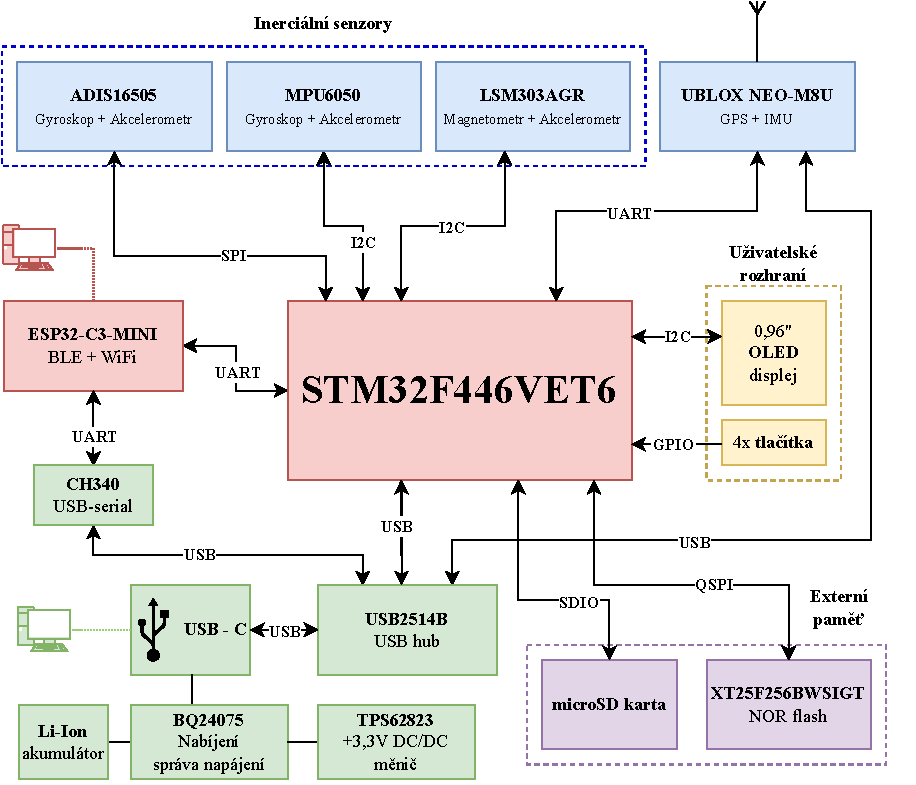
\includegraphics[width=\textwidth]{obrazky/IMUnav_H00_block}
    \caption{Blokové schéma inerciální jednotky}
\end{figure}

Hardware inerciální jednotky je realizován tak, aby umožňoval zaznamenávat hodnoty změřené inerciálními senzory a poskytovat dohromady data o rozměru 9~DoF (akcelerometr, gyroskop a magnetometr). Jednotka také obsahuje GPS modul s vestavěným IMU, jehož použití by mohlo být vhodné například v prostorech s alespoň částečným pokrytím signálu GPS.

Naměřená data je možné uložit do externí NOR Flash paměti připojené k MCU, popřípadě lze využít i kartu typu microSD. K přenosu dat pro jejich následné zpracování v PC primárně slouží ESP32-C3, umožňující bezdrátovou komunikaci přes Wifi, nebo Bluetooth. Konektor USB typu C umožňuje nabíjení vestavěného Li-Ion akumulátoru jednotky a komunikaci mezi PC a ESP32, GPS modulem a hlavním MCU skrze vestavěný USB rozbočovač. Toto rozhraní je plánované pro použití např. ke konfiguračním, nebo ladícím účelům.

Pro jednoduchou volnost pohybu je jednotka napájena jedním Li-Ion akumulátorem velikosti 18650, při záznamu dat tedy nebude potřeba externího zdroje energie. Grafický OLED displej a 4 tlačítka slouží jako uživatelské rozhraní při používání jednotky.

\subsection{Akcelerometr a gyroskop} \label{AccGyroText}
Jednotka obsahuje dvě 6~DoF IMU (gyroskop s akcelerometrem) rozdílných parametrů a řádově rozdílnou cenou. Takto odlišné součástky byly vybrány proto, aby bylo možné porovnat vliv přesnosti a šumu senzorů na následně zpracovaná data.
V Tabulce \ref{table:fyzikalniPorovnaniIMU} jsou porovnány důležité parametry senzorů MPU6050 a ADIS16505-2. Pro účely inerciální navigace je důležitý zejména nízký drift senzorů, aby při integraci dat k vyhodnocení polohy nebyla integrována i driftová chyba, což má za výsledek velmi nepřesné zpracování hodnot.

\begin{table}[h!]
\centering
\begin{tabular}{c||c c c}
\hline 
Model IMU & MPU6050 & ADIS16505-2 & jednotka \\ 
\hline
\hline 
\multicolumn{4}{c}{Parametry gyroskopů} \\
\hline
\hline
Dynamický rozsah  & \makecell{programovatelný, \\ $\pm 250$, $\pm 500$, \\$\pm 1000$, $\pm 2000$} & $\pm 500$ & $\SI[per-mode = symbol]{}{\degree\per\second}$ \\ 
\hline 
Citlivost  \tablefootnote{Pro porovnání citlivosti byl vybrán dynamický rozsah $\SI[per-mode = symbol]{500}{\degree\per\second}$ senzoru MPU6050 pro možnost porovnání hodnoty s druhým senzorem} & $65,5$ & $2621440$ & $\SI[per-mode = symbol]{}{\LSB\per(\degree\per\second)}$ \\ 
\hline 
Drift v ose x a z & $\pm 20$ & $\pm 0,14$ & $\SI[per-mode = symbol]{}{\degree\per\second}$ \\ 
\hline 
Drift v ose y & $\pm 20$ & $\pm 1,4$ & $\SI[per-mode = symbol]{}{\degree\per\second}$ \\ 
\hline 
\makecell{Efektivní hodnota hustoty \\šumu při 10Hz pro osy x a y} & 0,005 & 0,0043 & $\SI{}{\degree\per\second\per\sqrt{\Hz}}$ \\ 
\hline 
\makecell{Efektivní hodnota hustoty \\šumu při 10Hz pro osu z} & 0,005 & 0,0034 & $\SI{}{\degree\per\second\per\sqrt{\Hz}}$ \\ 
\hline 
\hline 
\multicolumn{4}{c}{Parametry akcelerometrů} \\
\hline
\hline
Dynamický rozsah  & \makecell{programovatelný, \\ $\pm 19,6$, $\pm 39,2$, \\$\pm 78,4$, $\pm 156,8$} & $\pm 78,4$ & $\SI[per-mode = symbol]{}{\metre\per\second\squared}$ \\ 
\hline 
Citlivost  \tablefootnote{Pro porovnání citlivosti byl vybrán dynamický rozsah $\SI[per-mode = symbol]{78,4}{\metre\per\second\squared}$ senzoru MPU6050 pro možnost porovnání hodnoty s druhým senzorem} & $418$ & $26756268$ & $\SI[per-mode = symbol]{}{\LSB\per(\metre\per\second\squared)}$ \\ 
\hline 
Drift v ose x a y & $\pm 0,491$ & $\pm 0,0196$ & $\SI[per-mode = symbol]{}{\metre\per\second\squared}$ \\ 
\hline 
Drift v ose z & $\pm 0,785$ & $\pm 0,0196$ & $\SI[per-mode = symbol]{}{\metre\per\second\squared}$ \\ 
\hline 
\makecell{Efektivní hodnota hustoty \\šumu při 10Hz pro osy x a y} & 3924 & 167 & $\SI{}{\micro\metre\per\second\squared\per\sqrt{\Hz}}$ \\ 
\hline 
\makecell{Efektivní hodnota hustoty \\šumu při 10Hz pro osu z} & 3924 & 243 & $\SI{}{\micro\metre\per\second\squared\per\sqrt{\Hz}}$ \\ 
\hline 

\end{tabular} 
\caption{Porovnání základních parametrů gyroskopů \cite{euxR3Yh5ol4JWNAi} \cite{UZFqHmQU7ZzI3OLB}} 
\label{table:fyzikalniPorovnaniIMU}
\end{table} 


Integrovaný obvod MPU6050 je standardní 6 osé MEMS IMU, vhodné mimo jiné pro použití v mobilních zařízeních a dalších podobných aplikacích. Jeho vnitřní gyroskop a akcelerometr má softwarově přepínatelné rozsahy měřených veličin. Kromě inerciálních senzorů má i vestavěný signálový procesor pro fúzi a filtrování dat přímo v integrovaném obvodu. Tato funkce může být vhodná pro odlehčení výpočetního výkonu hlavního procesoru, ovšem pro účely této práce nebude signálový procesor využit, jelikož se měřená data budou zpracovávat až po jejich naměření v PC, ne v reálném čase. Vzorkovací frekvence gyroskopu je 8 kHz a akcelerometru 1 kHz, oba senzory mají 16bitové rozlišení.
\cite{euxR3Yh5ol4JWNAi}

MPU6050 disponuje rozhraním I2C s maximální frekvencí hodinového signálu 400 kHz. \cite{euxR3Yh5ol4JWNAi}
Pokud bychom chtěli vyčítat ze senzoru data při maximální možné vzorkovací frekvenci, byla by potřeba minimální přenosová rychlost sběrnice:
$$ f_{clk}=3~\mathrm{osy} \times(f_{gyro} + f_{acc})\times (\mathrm{16bitů} + 2 \times \mathrm{ACK})=3\times(8000+1000)\times(16+2)=\SI{486}{\kilo\hertz}$$
Při vyčítání dat o maximální vzorkovací frekvenci jsme omezeni samotným I2C rozhraním senzoru (využití maximální vzorkovací frekvence je teoreticky možné krátkodobě, pomocí interního 1kB FIFO zásobníku).\cite{euxR3Yh5ol4JWNAi}

Jelikož pro účely inerciální navigace stačí vzorkovací frekvence dat v  řádu stovek~Hz \cite{Wei2022}, tak není tato limitace omezující. Senzor je propojen s hlavním MCU přes I2C sběrnici s frekvencí hodinového signálu 400 kHz a není sdílena s žádným jiným zařízením, aby bylo možné, v případě potřeby, využít maximální dostupný potenciál senzoru (i přestože je reálná potřeba vzorkovací frekvence nižší).

Integrovaný obvod ADIS16505-2 je precizní 6 osé MEMS IMU, vhodné pro použití v průmyslových a navigačních aplikacích s poměrně nízkým driftem a vysokou přesností. Na rozdíl od MPU6050 nemá přepínatelný dynamický rozsah, je fixně daný variantou součástky. Vzorkovací frekvence gyroskopu i akcelerometru je 2 kHz, oba senzory mají 32bitové rozlišení. S hlavním MCU komunikuje přes sběrnici SPI s maximální frekvencí hodinového signálu 2,1 Mhz. \cite{UZFqHmQU7ZzI3OLB} Pokud budeme chtít vyčítat data ze senzoru při maximální možné vzorkovací frekvenci, bude potřeba minimální přenosová rychlost sběrnice: 
$$ f_{clk}=3~\mathrm{osy} \times(f_{gyro} + f_{acc})\times \mathrm{32bitů}=3\times(2000+2000)\times 32=\SI{384}{\kilo\hertz}$$
Nejsme tedy omezeni maximální frekvencí hodinového signálu a můžeme teoreticky využívat senzor i při nejvyšší možné rychlosti.

Výrobce poskytuje tento obvod ve variantě 100 pinového BGA čipu, ale i jako vývojovou desku osazenou senzorem a kolíkovou lištou pro jednodušší práci s osazením DPS. \cite{UZFqHmQU7ZzI3OLB} Hardware jednotky byl navržen tak, aby bylo možné využít jak samotný BGA čip, tak i hotový modul s konektorem.

\subsection{Magnetometr}
Vzhledem k tomu, že výběr komerčně dostupných 9 DoF (akcelerometr, gyroskop a magnetometr) je značně omezený, popřípadě součástky prodávané jako 9osé IMU jsou ve skutečnosti moduly více součástek na jedné desce, tak je ve výsledném obvodovém zapojení použit senzor magnetické indukce jakožto samostatná součástka. 

Přestože fúze dat z magnetometru může mít pozitivní dopady na zmenšení chyby trajektorie \cite{Tkhorenko2018}, jeho použití uvnitř budov je značně omezené vzhledem k jednoduché ovlivnitelnosti měření blízkými feromagnetickými látkami, silovými rozvody elektřiny a pod. Proto nebyly na výběr magnetometru kladeny vysoké požadavky a slouží spíše pro porovnání vlivu přítomnosti / absence naměřených dat z tohoto senzoru.

K tomuto účelu byl vybrán běžně dostupný obvod LSM303AGR, který kromě magnetometru v pouzdře obsahuje i akcelerometr, ten ovšem nebude pro potřeby práce využit, jelikož tuto funkci obstarávají součástky z kapitoly \ref{AccGyroText}.

Magnetometr komunikuje s hlavním MCU přes sběrnici I2C s maximální vzorkovací frekvencí 150 Hz, dynamickým rozsahem $ \pm \SI{4.915}{\milli\tesla} $ a 16bitovým rozlišením. \cite{RD5DwZcremhT6bgp}



